\documentclass[11pt,letterpaper]{article}
\topmargin -.5truein
\textheight 9.0truein
\oddsidemargin 0truein
\evensidemargin 0truein
\textwidth 6.5truein
\setlength{\parskip}{5pt}
\setlength\parindent{0pt}
\usepackage[ruled,vlined]{algorithm2e}
\usepackage[table]{xcolor}% http://ctan.org/pkg/xcolor
\usepackage{caption}
\usepackage{subcaption}
\usepackage[round]{natbib}
\usepackage{graphicx}
\usepackage{amsmath}
\usepackage{amssymb}
\usepackage{wrapfig}
\usepackage{dsfont}
\usepackage{multirow}
\usepackage[all]{xy}
\usepackage{tikz}
\usepackage{tikz-qtree}


\DeclareMathOperator*{\argmax}{argmax}

\newcommand{\ra}{\ensuremath{\rightarrow}}
\newcommand{\bs}{\textbackslash}
%\renewcommand{\vec}[1]{\mathbf{#1}}
\newcommand{\vv}[1]{\ensuremath{\vec{\mathbf{#1}}}}

\newcommand{\ngramstart}{\ensuremath{\langle \textsc{s} \rangle}}
\newcommand{\ngramend}{\ensuremath{\langle \textsc{e} \rangle}}
\newcommand{\ngramunk}{\ensuremath{\langle unk \rangle}}

\newcommand{\wcurr}{\ensuremath{w_i}}
\newcommand{\tcurr}{\ensuremath{t_i}}
\newcommand{\tprev}{\ensuremath{t_{i-1}}}

\usepackage{hyperref}
\hypersetup{
    colorlinks,
    citecolor=black,
    filecolor=black,
    linkcolor=black,
    urlcolor=black
}

\title{NLP: Parsing}
\author{Dan Garrette\\\small{dhg@cs.utexas.edu}}

\begin{document}
\maketitle



\section{Grammar}

\vspace{-7mm}\Tree 
  [.S  
    [.NP [.D the ] [.N man ] ] 
    [.VP 
      [.V walks ] 
      [.NP [.D a ] [.N dog ] ] 
    ] 
  ]
\vspace{-2mm}
\begin{itemize}
  \item ``Consitiuency'' parse
  \item S (sentence), NP (noun phrase), VP (verb phrase) are constituents
  \item Words combine to make phrases, and phrases combine to make larger phrases and sentences.
\end{itemize}


\section{Context-Free Grammars (CFG)}

\begin{itemize}
  \item Context-free grammars can be specified by a table of ``productions''
	\begin{center}
	\begin{tabular}{llll p{10mm} lll}
	  S & $\ra$ & NP VP   &                                && D & $\ra$ & \{\textit{the, a}\}      \\
	    &       &         &                                &&   &       &                          \\
	  NP & $\ra$ & D N    & (``\underline{a dog} barks'')  && N & $\ra$ & \{\textit{man, dog}\}    \\
	  NP & $\ra$ & N      & (``\underline{dogs} bark'')    \\
	    &       &         &                                &&   &       &                          \\
	  VP & $\ra$ & V NP   & (transitive verb)              && V & $\ra$ & \{\textit{barks, walks, saw}\} \\
	  VP & $\ra$ & V      & (intransitive verb)
	\end{tabular}
	\end{center}
  \item Words are called ``terminals'' and other nodes are ``non-terminals''
  \item[]
  \item[]
  \item[]
  \item Independence assumption: each rule choice is dependent only on the parent node; it is independent of all other rule choices
  \item Independence assumption leads to many problems.  A couple:
	\begin{figure}[h]
	    \centering
        \begin{subfigure}[b]{0.5\textwidth}
          \begin{small} \Tree [.S [.NP [.D the ] [.N dog ] ] [.VP [.V \textbf{barks} ] [.NP [.D a ] [.N car ] ] ] ]
		  \end{small}
		  \caption{Intransitive verb with a direct object}
        \end{subfigure}
        \begin{subfigure}[b]{0.38\textwidth}
          \begin{small}
                \Tree [.S  [.NP [.D a ] [.N \textbf{dogs} ] ] [.VP [.V barks ] ] ] 
		  \end{small}
		  \caption{Noun doesn't agree in number with determiner or verb}
        \end{subfigure}
	\end{figure}
  \item We can solve some of these issues by refining our CFG.  For example:
	\begin{center}
	\begin{tabular}{llll p{10mm} lll}
	  VP & $\ra$ & IV      & (intransitive verb)            && IV & $\ra$ & \{\textit{barks, walks}\} \\
	  VP & $\ra$ & TV NP   & (transitive verb)              && TV & $\ra$ & \{\textit{chases, walks}\}
	\end{tabular}
	\end{center}
	\begin{figure}[h]
        \begin{subfigure}[b]{0.5\textwidth}
          \begin{small} \Tree [.S [.NP [.D the ] [.N dog ] ] [.VP [.\textbf{TV} \textbf{chases} ] [.NP [.D a ] [.N car ] ] ] ] \end{small}
		  \caption{Intransitive verbs are disallowed}
        \end{subfigure}
        \begin{subfigure}[b]{0.38\textwidth}
          \begin{small} \Tree [.S [.NP [.D the ] [.N dog ] ] [.VP [.\textbf{IV} \textbf{barks} ] ] ] \end{small}
		  \caption{Transitive verbs are disallowed}
        \end{subfigure}
	\end{figure}

\end{itemize}

\newpage
\section{Syntactic Ambiguity}

\begin{itemize}
  \item For a given CFG, there can be multiple trees that describe the same sentence
  \item Add the following rules to the above:
	\begin{center}
	\begin{tabular}{llll p{10mm} lll}
	  NP & $\ra$ & D N PP    & (prep phrase attach to noun)  &&  N & $\ra$ & \{\textit{telescope}\}    \\
	  VP & $\ra$ & V NP PP   & (prep phrase attach to verb)  &&   \\
	  PP & $\ra$ & P NP      & (``in the house'')  &&   
	\end{tabular}
	\end{center}
  \item ``The man saw a dog with a telescope''
	\begin{figure}[h]
	    \centering
		\begin{subfigure}[b]{0.5\textwidth}
		  \begin{small}
		        \Tree 
				  [.S  
				    [.NP [.D the ] [.N man ] ] 
				    [.VP 
				      [.V saw ] 
				      [.NP [.D a ] [.N dog ] ] 
				      [.PP [.P with ] [.NP [.D a ] [.N telescope ] ] ]
				    ] 
				  ]
		  \end{small}
		\end{subfigure}
		\begin{subfigure}[b]{0.3\textwidth}
		  \begin{small}
		        \Tree 
				  [.S  
				    [.NP [.D the ] [.N man ] ] 
				    [.VP 
				      [.V saw ] 
				      [.NP 
				        [.D a ] [.N dog ] 
				        [.PP [.P with ] [.NP [.D a ] [.N telescope ] ] ]
				      ] 
				    ] 
				  ]
		  \end{small}
		\end{subfigure}
	\end{figure}

  \item Ambiguity is explosive
  \item A sentence ending in $n$ prepositional phrases has \textit{over} $2^n$ parses (catalan numbers)
	\begin{itemize}
	  \item ``I saw the man with the telescope'': 2 parses
	  \item ``I saw the man on the hill with the telescope'': 5 parses
	  \item ``I saw the man on the hill in texas with the telescope'': 14 parses
	  \item ``I saw the man on the hill in texas with the telescope at noon'': 42 parses
	  \item ``I saw the mon on the hill in texas with the telescope at noon on monday'': 132 parses
	\end{itemize}
\end{itemize}



\section{Agreement}

\begin{itemize}
  \item In order for a sentence to be grammatical, we must also respect \textit{agreement rules} 
	\begin{itemize}
	  \item number: \textit{a dog} vs. \textit{all dogs}
	  \item person: 1st person (\textit{I am}), 2nd person (\textit{you are}), 3rd person (\textit{he is})
	  \item gender: \textit{un homme} vs. \textit{use femme} or even \textit{she sees herself}
	\end{itemize}

  \item[]
  \item The grammar defined above does not enforce this
	\begin{itemize}
	  \item For an NP, since productions are independent of each other, we could get either \textit{dog} or \textit{dogs} no matter whether the D is \textit{a} or \textit{all}
	\end{itemize}

  \item We can incorporate this into our grammar by duplicating our productions to ensure agreement:
	\begin{center}
	\begin{tabular}{llll p{8mm} lll}
	  S & $\ra$ & NP$_{\text{sg}}$ VP$_{\text{sg}}$                &                                         && D$_{\text{sg}}$ & $\ra$ & \{\textit{the, a}\}      \\
	  S & $\ra$ & NP$_{\text{pl}}$ VP$_{\text{pl}}$                &                                         && D$_{\text{pl}}$ & $\ra$ & \{\textit{the, all}\}    \\
	  \\
	  NP$_{\text{pl}}$ & $\ra$ & N$_{\text{pl}}$                   & (``\underline{dogs} bark'')             && N$_{\text{sg}}$ & $\ra$ & \{\textit{dog}\}    \\
	  NP$_{\text{pl}}$ & $\ra$ & D$_{\text{pl}}$ N$_{\text{pl}}$   & (``\underline{all dogs} bark'')         && N$_{\text{pl}}$ & $\ra$ & \{\textit{dogs}\}    \\
	  NP$_{\text{sg}}$ & $\ra$ & D$_{\text{sg}}$ N$_{\text{sg}}$   & (``\underline{a dog} barks'')    \\
	  \\
	  VP$_{\text{sg}}$ & $\ra$ & V$_{\text{sg}}$                   & (``a dog \underline{barks}'')           && V$_{\text{sg}}$ & $\ra$ & \{\textit{barks, walks, sees}\} \\
	  VP$_{\text{sg}}$ & $\ra$ & V$_{\text{sg}}$ NP$_{\text{sg}}$  & (``a dog \underline{chases a car}'')    && V$_{\text{pl}}$ & $\ra$ & \{\textit{bark, walk, see}\} \\
	  VP$_{\text{sg}}$ & $\ra$ & V$_{\text{sg}}$ NP$_{\text{pl}}$  & (``a dog \underline{chases cars}'')     && \\
	  \\
	  VP$_{\text{pl}}$ & $\ra$ & V$_{\text{pl}}$                   & (``all dogs \underline{bark}'')         && \\
	  VP$_{\text{pl}}$ & $\ra$ & V$_{\text{pl}}$ NP$_{\text{sg}}$  & (``all dogs \underline{chase a car}'')  && \\
	  VP$_{\text{pl}}$ & $\ra$ & V$_{\text{pl}}$ NP$_{\text{pl}}$  & (``all dogs \underline{chase cars}'')   &&
	\end{tabular}
	\end{center}

  \item But this quickly explodes the number of rules
  \item And the explosion is worse with more agreement rules:
	\begin{center}
	\begin{tabular}{llll p{8mm} lll}
	  VP$_{\text{sg,1st,masc}}$ & $\ra$ & V$_{\text{sg,1st,masc}}$            \\
	  VP$_{\text{sg,1st,fem}}$ & $\ra$ & V$_{\text{sg,1st,fem}}$            \\
	  VP$_{\text{sg,2nd,masc}}$ & $\ra$ & V$_{\text{sg,2nd,masc}}$            \\
	  VP$_{\text{sg,2nd,fem}}$ & $\ra$ & V$_{\text{sg,2nd,fem}}$            \\
	  ... \\
	  VP$_{\text{pl,3rd,fem}}$ & $\ra$ & V$_{\text{pl,3rd,fem}}$            \\
	\end{tabular}
	\end{center}

  \item We can simplify this greatly using \textit{feature structures} that use variables to ensure agreement
	\begin{center}
	\begin{tabular}{llll p{8mm} lll}
	  S & $\ra$ & NP$_{\text{[num=$x$]}}$ VP$_{\text{[num=$x$]}}$                         &   && D$_{\text{[num=sg]}}$ & $\ra$ & \{\textit{a, every}\}      \\
	    &       &                                                                         &   && D$_{\text{[num=pl]}}$ & $\ra$ & \{\textit{all, some}\}      \\
	  NP$_{\text{[num=$x$]}}$ & $\ra$ & D$_{\text{[num=$x$]}}$ N$_{\text{[num=$x$]}}$     &   && D$_{\textbf{[num=$z$]}}$ & $\ra$ & \{\textit{the}\}      \\
	    &       &                                                                         &   \\
	  VP$_{\text{[num=$x$]}}$ & $\ra$ & V$_{\text{[num=$x$]}}$                            &   && N$_{\text{[num=sg]}}$ & $\ra$ & \{\textit{dog}\}      \\
	  VP$_{\text{[num=$x$]}}$ & $\ra$ & V$_{\text{[num=$x$]}}$ NP$_{\textbf{[num=$y$]}}$  &   && N$_{\text{[num=pl]}}$ & $\ra$ & \{\textit{dogs}\}      \\
	  \\
	    &       &                                                                         &   && V$_{\text{[num=sg]}}$ & $\ra$ & \{\textit{barks, walks, sees}\} \\
	    &       &                                                                         &   && V$_{\text{[num=pl]}}$ & $\ra$ & \{\textit{bark, walk, see}\} \\
	\end{tabular}
	\end{center}

  \item[]
  \item[]
  \item[]
  \item Feature structures must \textit{unify} as they are combined
	\begin{itemize}
	  \item For example, all $x$s and $z$ must resolve to the same value (\textit{sg} or \textit{pl})
	\end{itemize}

	\begin{figure}[h]
	    \centering
		\begin{subfigure}[t]{0.4\textwidth}
		  \begin{small}
		    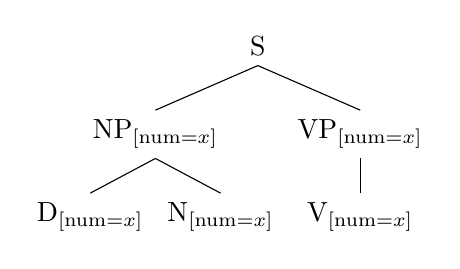
\begin{tikzpicture}[]
			\Tree 
			  [.S  
			    [.NP$_{\text{[num=$x$]}}$ 
			      [.D$_{\text{[num=$x$]}}$ ] 
			      [.N$_{\text{[num=$x$]}}$ ] ] 
			    [.VP$_{\text{[num=$x$]}}$  
			      [.V$_{\text{[num=$x$]}}$ ] ] 
			  ]
			\end{tikzpicture}
		    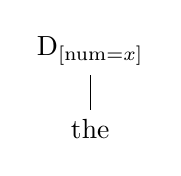
\begin{tikzpicture}[]
			\Tree 
			  [.D$_{\text{[num=$x$]}}$ the ]
			\end{tikzpicture}
		    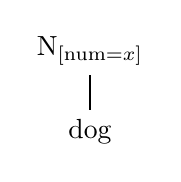
\begin{tikzpicture}[]
			\Tree 
			  [.N$_{\text{[num=$x$]}}$ dog ]
			\end{tikzpicture}
		    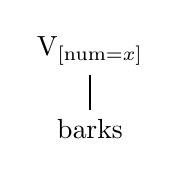
\begin{tikzpicture}[]
			\Tree 
			  [.V$_{\text{[num=$x$]}}$ barks ]
			\end{tikzpicture}
		  \end{small}
		  \caption{Need to unify underspecified features in the rules with secified features in the N and V terminal rules}
		\end{subfigure}
		~~~~~
		\begin{subfigure}[t]{0.3\textwidth}
		  \begin{small}
			\Tree 
			  [.S  
			    [.NP$_{\text{[num=sg]}}$ [.D$_{\text{[num=sg]}}$ the ] [.N$_{\text{[num=sg]}}$ dog ] ] 
			    [.VP$_{\text{[num=sg]}}$ [.V$_{\text{[num=sg]}}$ barks ] ] 
			  ]
		  \end{small}
		  \caption{all $x$s and $z$ resolve to ``sg''}
		\end{subfigure}
	\end{figure}

  \item Similar features could be set up for other required agreements
	\begin{itemize}
	  \item PRO[num=sg, per=3rd, gen=masc] $\rightarrow$ \textit{il}
	\end{itemize}
\end{itemize}



\section{Probabilistic Context-Free Grammars (PCFG)}

\begin{itemize}
  \item A CFG is deterministic
	\begin{itemize}
	  \item It can decide whether a sentence is in the language (grammatical), or not
	  \item It can't judge whether one sentence is more likely than another
	  \item Problematic since we want to say that every sentence is \textit{possible}, even if it's not likely
	\end{itemize}
  \item A PCFG is a CFG in which, for every non-terminal, we have a probability distribution over possible productions
  \item In other words, for each non-terminal A, we have a distribution $p(\beta \mid A)$
	\begin{itemize}
	  \item The probability that, given a parent non-terminal A, we choose the production rule that yields $\beta$
	  \item We can alternatively write this as $p(A \ra \beta)$
	\end{itemize}
\end{itemize}

	\begin{center}
	\begin{tabular}{llll p{18mm} llll}
	  S  & $\ra$ & NP VP    &  1.0  &&  D & $\ra$ & \textit{the}        & 0.6 \\
	     &       &          &       &&  D & $\ra$ & \textit{a}          & 0.4 \\
	  NP & $\ra$ & D N      &  0.7  &&    &       &                     &     \\
	  NP & $\ra$ & N        &  0.2  &&  N & $\ra$ & \textit{man}        & 0.5 \\
	  NP & $\ra$ & D N PP   &  0.1  &&  N & $\ra$ & \textit{dog}        & 0.4 \\
	     &       &          &       &&  N & $\ra$ & \textit{telescope}  & 0.1 \\
	  VP & $\ra$ & V NP     &  0.4  &&    &       &                     &     \\
	  VP & $\ra$ & V        &  0.4  &&  V & $\ra$ & \textit{barks}      & 0.2 \\
	  VP & $\ra$ & V NP PP  &  0.2  &&  V & $\ra$ & \textit{walks}      & 0.4 \\
	     &       &          &       &&  V & $\ra$ & \textit{saw}        & 0.4
	\end{tabular}
	\end{center}

\vspace{-5mm}
Estimating parameters (MLE)

\begin{itemize}
  \item We can calculate the MLE parameters of a PCFG model by counting productions in a corpus of parse trees
  \item Assume these three sentences comprise a corpus:
	\begin{figure}[h]
	        \centering
	        \begin{subfigure}[b]{0.25\textwidth}
	          \begin{small} \Tree [.S [.NP [.D the ] [.N dog ] ] [.VP [.V ran ] ] ] \end{small}
	        \end{subfigure}
	        \begin{subfigure}[b]{0.4\textwidth}
	          \begin{small} \Tree [.S  [.NP [.D the ] [.N man ] ] [.VP [.V walked ] [.NP [.D a ] [.N dog ] ] ] ] \end{small}
	        \end{subfigure}
	        \begin{subfigure}[b]{0.2\textwidth}
	          \begin{small} \Tree [.S  [.NP [.D the ] [.N man ] ] [.VP [.V walked ] ] ] \end{small}
	        \end{subfigure}
	\end{figure}
	\vspace{-5mm}
  \item We estimate by counting up all productions in the corpus and normalizing
    \begin{itemize}
      \item Since every non-terminal $A$ must produce \textit{something}, we can simplify slightly
    \end{itemize}
    \[ p(\beta \mid A) = \frac{C(A \ra\beta)}{\sum_{\beta' \in P} C(A \ra\beta')} = \frac{C(A \ra\beta)}{C(A)} \]
  \item Estimates from the above corpus of trees yield: \vspace{-3mm}
	\begin{center}
	\begin{tabular}{lllcc p{13mm} lllcc}
	     &       &          & $C(A\ra\beta)$ & $p(\beta\mid A)$ &&    &       &                   & $C(A\ra\beta)$ & $p(\beta\mid A)$ \\
	  \hline
	  S  & $\ra$ & NP VP    &  3             & 1.0              &&  D & $\ra$ & \textit{the}      & 3              & 0.75             \\
	     &       &          &                &                  &&  D & $\ra$ & \textit{a}        & 1              & 0.25             \\
	  NP & $\ra$ & D N      &  4             & 1.0              &&    &       &                   &                &                  \\
	     &       &          &                &                  &&  N & $\ra$ & \textit{dog}      & 2              & 0.5              \\
	  VP & $\ra$ & V        &  2             & 0.66             &&  N & $\ra$ & \textit{man}      & 2              & 0.5              \\
	  VP & $\ra$ & V NP     &  1             & 0.33             \\
	     &       &          &                &                  &&  V & $\ra$ & \textit{walked}   & 2              & 0.66             \\
	     &       &          &                &                  &&  V & $\ra$ & \textit{ran}      & 1              & 0.33             
	\end{tabular}
	\end{center}
\end{itemize}


Add-$\lambda$ smoothing

\begin{itemize}
  \item Same as always (where $P$ is the set of all possible $\beta$s produced):
    \[ p(\beta \mid A) 
      = \frac{C(A \ra\beta)+\lambda}{\sum_{\beta' \in P} (C(A \ra\beta')+\lambda)} 
      = \frac{C(A \ra\beta)+\lambda}{(\sum_{\beta' \in P} C(A \ra\beta'))+\lambda|P|} 
      = \frac{C(A \ra\beta)+\lambda}{C(A)+\lambda|P|} \]
\end{itemize}


Likelihood of a (parsed) sentence

\begin{itemize}
  \item We can use this to calculate the likelihood of seeing a particular parse of a particular sentence
  \item Multiply the probabilities of all productions found in the tree
  \item Assume this tree:
	\begin{small} \Tree [.S [.NP [.D the ] [.N dog ] ] [.VP [.V walked ] [.NP [.D a ] [.N man ] ] ] ] \end{small}
  \item Count up the number of each production in the tree, and get the probability of each production from the above table
	\begin{center}
	\begin{tabular}{lllcc p{13mm} lllcc}
	     &       &          & count & prob  &&    &       &                   & count & prob \\
	  \hline
	  S  & $\ra$ & NP VP    &  1    & 1.0   &&  D & $\ra$ & \textit{the}      & 1     & 0.75             \\
	     &       &          &       &       &&  D & $\ra$ & \textit{a}        & 1     & 0.25             \\
	  NP & $\ra$ & D N      &  2    & 1.0   &&    &       &                   &       &                  \\
	     &       &          &       &       &&  N & $\ra$ & \textit{dog}      & 1     & 0.5              \\
	  VP & $\ra$ & V NP     &  1    & 0.33  &&  N & $\ra$ & \textit{man}      & 1     & 0.5              \\
	     &       &          &       &       \\
	     &       &          &       &       &&  V & $\ra$ & \textit{walked}   & 1     & 0.66             \\
	\end{tabular}
	\end{center}
  \item Find the product:
    \begin{align*}
      & p(\text{S}\ra\text{NP VP}) \cdot
        p(\text{NP}\ra\text{D N})^{2} \cdot
        p(\text{VP}\ra\text{V NP}) \cdot
        p(\text{D}\ra\textit{the}) \cdot
        p(\text{D}\ra\textit{a}) \cdot
        p(\text{N}\ra\textit{dog}) \\&~~~\cdot
        p(\text{N}\ra\textit{man}) \cdot
        p(\text{V}\ra\textit{walked}) \\
      &= 1.0 \cdot 1.0^{2} \cdot 0.33 \cdot 0.75 \cdot 0.25 \cdot 0.5 \cdot 0.5 \cdot 0.66
    \end{align*}
	\item Note that the $p(\text{NP}\ra\text{D N})$ term is squared since the production ``$\text{NP}\ra\text{D N}$'' appears twice in the tree
\end{itemize}




\section{Lexicalized Grammars}

\begin{itemize}
  \item Problem: trees do not take semantic coherence into account
  \item Production rules are independent
  \item These two sentence have \textit{exactly} the same likelihood
	\begin{figure}[h]
        \centering
        \begin{subfigure}[b]{0.5\textwidth}
		  \begin{small} \Tree [.S [.NP [.D the ] [.N \textbf{dog} ] ] [.VP [.V bit ] [.NP [.D a ] [.N \textbf{man} ] ] ] ] \end{small}
        \end{subfigure}
        \begin{subfigure}[b]{0.3\textwidth}
		  \begin{small} \Tree [.S [.NP [.D the ] [.N \textbf{man} ] ] [.VP [.V bit ] [.NP [.D a ] [.N \textbf{dog} ] ] ] ] \end{small}
        \end{subfigure}
	\end{figure}
  \item Since it's a product, we can swap two productions without changing the result
	\begin{small}
    \[
       p(\text{S}\ra\text{NP VP}) \cdot
        p(\text{NP}\ra\text{D N})^{2} \cdot
        p(\text{VP}\ra\text{V NP}) \cdot
        p(\text{D}\ra\textit{the}) \cdot
        p(\text{D}\ra\textit{a}) \cdot
        \mathbf{p(\textbf{N}\ra\textbf{\textit{dog}})} \cdot
        \mathbf{p(\textbf{N}\ra\textbf{\textit{man}})} \cdot
        p(\text{V}\ra\textit{bit}) 
        \vspace{-2.5mm}\]
        \hspace{4.5in}$\mathbf{\downarrow}$\hspace{0.8in}$\mathbf{\downarrow}$
        \vspace{-2mm}
    \[ p(\text{S}\ra\text{NP VP}) \cdot
        p(\text{NP}\ra\text{D N})^{2} \cdot
        p(\text{VP}\ra\text{V NP}) \cdot
        p(\text{D}\ra\textit{the}) \cdot
        p(\text{D}\ra\textit{a}) \cdot
        \mathbf{p(\textbf{N}\ra\textbf{\textit{man}})} \cdot
        \mathbf{p(\textbf{N}\ra\textbf{\textit{dog}})} \cdot
        p(\text{V}\ra\textit{bit}) \]
    \end{small}
  \item Solution: lexicalize the grammar
  \item Subcategorize rules with their head words:
	\begin{center}
	\begin{tabular}{llll p{18mm} llll}
	  S  & $\ra$ & NP(man) VP(bite)            &  0.3  &&  D & $\ra$ & \textit{the}        & 0.6 \\
	  S  & $\ra$ & NP(dog) VP(bite)            &  0.7  &&  D & $\ra$ & \textit{a}          & 0.4 \\
	  S$^1$  & $\ra$ & NP(sandwich) VP(bite)       &  0.0  &&    &       &                     &     \\
	     &       &                             &       &&    &       &                     &     \\
	  NP(man)$^2$ & $\ra$ & D N(man)               &  0.8  &&  N(man)$^2$ & $\ra$ & \textit{man}   & 0.7 \\
	  NP(man)$^2$ & $\ra$ & N(man)                 &  0.2  &&  N(man)$^2$ & $\ra$ & \textit{men}   & 0.3 \\
	     &       &                             &       &&    &       &                     &     \\
	  NP(dog)$^3$ & $\ra$ & D N(dog)               &  0.4  &&  N(dog)$^3$ & $\ra$ & \textit{dog}   & 0.2 \\
	  NP(dog)$^3$ & $\ra$ & N(dog)                 &  0.6  &&  N(dog)$^3$ & $\ra$ & \textit{dogs}  & 0.8 \\
	     &       &                             &       &&    &       &                     &     \\
	  VP(bite)$^4$ & $\ra$ & V(bite) NP(man)       &  0.2  &&  V(bite) & $\ra$ & \textit{bite}    & 0.3 \\
	  VP(bite)$^4$ & $\ra$ & V(bite) NP(dog)       &  0.1  &&  V(bite) & $\ra$ & \textit{bites}   & 0.2 \\
	  VP(bite)$^4$ & $\ra$ & V(bite) NP(sandwich)  &  0.7  &&  V(bite) & $\ra$ & \textit{biting}  & 0.1 \\
	  VP(bite)$^5$ & $\ra$ & V(bite)               &  0.0  &&  V(bite) & $\ra$ & \textit{bit}     & 0.4 \\
	\end{tabular}
	\end{center}
  \begin{itemize}
    \item {}$^1$Sandwiches don't bite
    \item {}$^2$Men are likely talked about in the singular
    \item {}$^3$Dogs are likely talked about in the plural
    \item {}$^4$Men are bitten infrequently, dogs are bitten less frequently, and sandwiches are bitten often.
    \item {}$^5$``Biting'' can't be intransitive
  \end{itemize}

	\begin{figure}[h]
	        \centering
	        \begin{subfigure}[b]{0.5\textwidth}
	          \begin{small}
	                \Tree 
					  [.S  
					    [.NP(dog) [.D the ] [.N(dog) \textbf{dog} ] ] 
					    [.VP(bite) 
					      [.V(bite) bit ] 
					      [.NP(man) [.D a ] [.N(man) \textbf{man} ] ] 
					    ] 
					  ]
			  \end{small}
			  \caption{more likely}
	        \end{subfigure}
	        \begin{subfigure}[b]{0.3\textwidth}
	          \begin{small}
	                \Tree 
					  [.S  
					    [.NP(man) [.D the ] [.N(man) \textbf{man} ] ] 
					    [.VP(bite) 
					      [.V(bite) bit ] 
					      [.NP(dog) 
					        [.D a ] [.N(dog) \textbf{dog} ] 
					      ] 
					    ] 
					  ]
			  \end{small}
			  \caption{unlikely}
	        \end{subfigure}
	\end{figure}

  \item Downside: increased sparsity!
\end{itemize}


\section{Generative Model}

\begin{itemize}
  \item Like na\"{i}ve Bayes models, N-Gram models, and hidden Markov models
  \item Two probability distribution: $p(\beta \mid \alpha)$, for production rules $\alpha \ra \beta$, and $p(\sigma)$, where $\sigma$ is a possible ``start'' symbol
  \item Generative story:
    \begin{enumerate}
      \item Choose a start symbol $x$ from the distribution over start symbols $p(\sigma)$
      \item If $x$ is a terminal, STOP
      \item Else, choose some $\beta$ from $p(\beta \mid x)$
      \item ~~~For each symbol $y$ in $\beta$, go to step 2
    \end{enumerate}
  \item For each node with symbol $x$, we choose a production rule of the form $x \ra \beta$ according to their probabilities and then recursively choose rules for every node in $\beta$ until we reach terminals for all branches.
\end{itemize}



\section{Parsing}

Top-Down
\begin{itemize}
  \item Never try to build tree that doesn't make a sentence.
  \item Waste time exploring trees that don't end up with the correct words.
\end{itemize}

Bottom-Up
\begin{itemize}
  \item Never make a tree that doesn't start with the right words.
  \item Waste time exploring trees that don't make a sentence.
\end{itemize}


\section{Parsing with P-CKY}

Find the mostly likely parse tree $t$ for the sentence $w_0...w_n$
\begin{itemize}
  \item $ \hat{t} = \text{argmax}_t~p(t \mid w_0...w_n) $
  \item Since we know how to find the likelihood of a parse (from above), we could enumerate all possible trees, and find the likelihood of each one.
  \item But the number of possible trees is enormous
  \item We will use a \textit{dynamic programming} algorithm to find the best parse tree: P-CKY
  \item Probabilistic version of the CKY algorithm, which can be used with any CFG
  \item Analgous to the Viterbi algorithm (both are dynamic programming algorithms)
\end{itemize}

Chomsky Normal Form (CNF)
\begin{itemize}
  \item CKY requires that the grammar be in CNF
  \item All productions must be one of:
	\begin{itemize}
	  \item Non-terminal producing exactly 2 non-terminals: A \ra\ B C\\
	        Non-terminal producing exactly 1 non-terminal: A \ra\ B\\
	        Non-terminal producing exactly 1 terminal: A \ra\ \textit{w}
	\end{itemize}
  \item Any CFG can be convered to CNF
	\begin{itemize}
	  \item Producing more than two nonterminals: ``A \ra\ B ... Y Z'' becomes
		\begin{itemize}
		  \item A \ra\ B ... [Y+Z] \\ $[$Y+Z$]$ \ra\ Y Z
		  \item Repeat as necessary until you just have  A \ra\ B X
		  \item NP \ra\ D Adj N becomes\\  NP \ra\ D $[$Adj+N$]$ \\ $[$Adj+N$]$ \ra\ Adj N
		\end{itemize}
	  \item For our trees we should never have terminals and nonterminals mixed in productions since all terminals a produced by unary rules from POS tags, which never produce anything other than terminals. (But if we needed to we could create dummy non-terminals for those terminals.)
	\end{itemize}
\end{itemize}


P-CKY Idea

\begin{enumerate}
  \item Make a pass over the whole sentence, trying to find subtrees that explain spans within the sentence
  \item Dynamic programming: store intermediate results in a chart
  \item Start with the leftmost word.  For each non-terminal (NT), find the most plausible subtree that covers just that word.
  \item Move to the next word
    \begin{enumerate}
	  \item[a.] Again, for each NT, find the most plausible subtree that covers just that word.
	  \item[b.] Then, for each NT, find the most plausible subtree that covers both the word and the previous word.
	  \item[c.] Same for the three-word span of the word and the previous two words.
	  \item[d.] Continue until you have the entire span from the beginning of the sentence to the word.
	  \item[e.] Then move to the next word and repeat.
    \end{enumerate}
  \item You are finished when you have, for each NT, the most plausible tree covering the entire span of the sentence.
  \item Pick the root node that is most plausible considering the \textit{a priori} probability of an NT being the root of a sentence.
\end{enumerate}



P-CKY Algorithm


\begin{itemize}
  \item NT is the set of all non-terminals (including composites and POS tags)
  \item $N$ = length of sentence $w_0...w_{N-1}$
  \item \texttt{table[i,j][A]} is the best possible score for a subtree spanning words $w_i...w_{j-1}$ with $A$ as its root
  \item \texttt{back[i,j][A] = (k,B,C)} indicates that the best possible subtree spanning words $w_i...w_{j-1}$ with $A$ as its root is comprised of a left subtree spanning words $w_i...w_{k-1}$ with $B$ as its root and a right subtree spannign words $w_k...w_{j-1}$ with $C$ as its root.
\end{itemize}

\begin{algorithm}[h]
Initialize \texttt{table} to be an N+1 x N+1 array (for (best-so-far) scores) \\
Initialize \texttt{back} to be an N+1 x N+1 array (for backpointers) \\
\BlankLine
\For{$j \leftarrow 1$ \KwTo $N$}{
  \BlankLine
  \textit{// Fill in the bottom of the chart (single-word spans):} \\
    $i = j-1$ \;
    \For{$A \leftarrow$ \text{NT (or restrict to just POS tags if convenient)}}{
      \textit{// A is a potential POS tag for $w_i$} \\
      \If{$p(w_i \mid A) > 0.0$}{
         \textit{// $A \rightarrow w_i$ is a valid rule} \\
         \texttt{table[i,j][a]} = $p(w_i \mid A)$ \\
         \texttt{back[i,j][a]} = $w_i$ \\
      }
    }
  \BlankLine
  \textit{// Fill in the higher levels of the chart (multi-word spans)} \\
  \For{$i \leftarrow j$-1 \textbf{downto} 0}{
    \BlankLine
    \textit{// Binary Rules (with $k$ as pivot)} \\
    \For{$k \leftarrow i$+1 \KwTo $j$-1}{
	  \For{$B \leftarrow$ \texttt{table[i,k]} and $C \leftarrow$ \texttt{table[k,j]}}{	    
	    \textit{// B is the root of a sub-tree covering the span $w_i...w_{k-1}$} \\
	    \textit{// C is the root of a sub-tree covering the span $w_k...w_{j-1}$} \\
	    \For{$A \leftarrow$ \text{NT (or restrict to just non-POS tags if convenient)}}{
	      \textit{// A is a potential root for the subtree spanning $w_i...w_{j-1}$} \\
	      \If{$p(B~C \mid A) > 0.0$}{
	        \textit{// $A \rightarrow B~C$ is a valid rule} \\
	        $s = p(B~C \mid A)~\cdot $ \texttt{table[i,k][B]} $ \cdot $ \texttt{table[k,j][C]} \\
	        \If{\texttt{table[i,j]} doesn't contain $A$ \textbf{OR} \texttt{table[i,j][A]} $< s$}{
	          \textit{// Either we haven't seen a valid subtree coverting i to j with root A, } \\
	          \textit{// ~~or this new subtree has a higher score} \\
	          \texttt{table[i,j][A]} = $s$ \\
	          \texttt{back[i,j][A]} = $(k,B,C)$ \\
	        }
	      }
	    }
	  }
	}
	\BlankLine
	\textit{// Unary Rules} \\
	done = false \\
	\While{!done}{
	  done = true \\
	  \For{$B \leftarrow$ \texttt{table[i,j]}}{
	      \textit{// B is the root of a sub-tree covering the span $w_i...w_{j-1}$} \\
	      \For{$A \leftarrow$ \text{NT (or restrict to just non-POS, non-compound tags if convenient)}}{
	        \textit{// A is a potential root for the subtree spanning $w_i...w_{j-1}$} \\
	        \If{$p(B \mid A) > 0.0$}{
	          \textit{// $A \rightarrow B$ is a valid rule} \\
	          $s = p(B \mid A)~\cdot $ \texttt{table[i,j][B]} \\
	          \If{\texttt{table[i,j]} doesn't contain $A$ \textbf{OR} \texttt{table[i,j][A]} $< s$}{
	            \textit{// Either we haven't seen a valid subtree coverting i to j with root A, } \\
	            \textit{// ~~or this new subtree has a higher score} \\
	            \texttt{table[i,j][A]} = $s$ \\
	            \texttt{back[i,j][A]} = $B$ \\
	            done = false \textit{ // if we added a new NT, then re-check} \\
	          }
	        }
	      }
	    }
	  }
  }
}
\caption{P-CKY}
\end{algorithm}

\begin{algorithm}[h]
\BlankLine
\textit{// Select the best root element while considering the prior over all potential root elements} \\
root = $\displaystyle\argmax_{\substack{S \leftarrow \texttt{table[0,N]}}}$
           \texttt{table[0,N][S]}~$\cdot~p(S)$

\BlankLine
\eIf{\texttt{table[0,N][root]}~$\cdot~p(root) = 0.0$}{
  \textit{// There is no valid parse of the sentence}
}{
  FollowBackpointers(root, 0, N)
}


\BlankLine
\BlankLine
\BlankLine
\BlankLine
\textbf{Function} FollowBackpointers(A, i, j) : Tree \\
  \BlankLine
  ~~~~\texttt{back[i,j][A]} \textbf{match} \\
  ~~~~~~~~\textbf{case} (k, B, C)  $\Rightarrow$ ~~~~ // Binary branch \\
  ~~~~~~~~~~~~Tree(A, FollowBackpointers(B, i, k), FollowBackpointers(C, k, j)) \\
  ~~~~~~~~\textbf{case} B   $\Rightarrow$ ~~~~ // Unary branch \\
  ~~~~~~~~~~~~Tree(A, FollowBackpointers(B, i, j)) \\
  ~~~~~~~~\textbf{case} $w$ $\Rightarrow$ ~~~~ // Terminal (word) \\
  ~~~~~~~~~~~~Leaf($w$)
\caption{Retrieve the best-parse tree from the backpointer table}
\end{algorithm}


\section{P-CKY Example}

``the complex houses married students''

NP[the complex houses] VP[V[married] NP[N[students]]] \\
NP[this complex] VP[V[houses] [NP[A[married] [N students]]]
 


\section{N-Best Parses}

Useful for providing multiple possiblities to down-stream applications.

Can be fed into a discriminative re-ranker that uses something like MaxEnt with features built from linguistic knowlege to re-score the parses.  The discriminative model wouldn't be used for \textit{parsing}, just to calculate the likelihoods of the parses that were found.




\section{Other Grammatical Formalisms}

\subsection{TAG: Tree-Adjoining Grammar}

\begin{itemize}
  \item http://www.seas.upenn.edu/$\sim$joshi/joshi-schabes-tag-97.pdf
  \item Instead of single-layer production rules of a CFG, production rules are tree \textit{fragments}
  \item Fragments have ``incomplete'' nodes that must produce to other tree fragments. (Just like how ``incomplete'' nodes in a CFG must produce the next rule.)
  \item Lexicalized: Each fragment centered around a word
  \item Mildly context-sensitive (as opposed to context-free)
\end{itemize}

\begin{figure}[h]
  \centering
  \begin{subfigure}[b]{0.2\textwidth}
  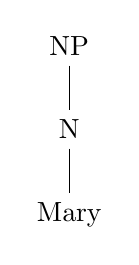
\begin{tikzpicture}
    \Tree 
      [.NP [.N [.Mary ] ] ] 
  \end{tikzpicture}
  \end{subfigure}
  \begin{subfigure}[b]{0.30\textwidth}
  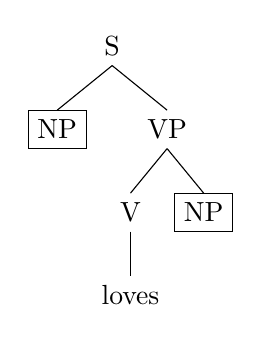
\begin{tikzpicture}
    \Tree 
      [.S 
        [.\node[draw]{NP}; ] 
        [.VP 
          [.V [.loves ] ] 
          [.\node[draw]{NP}; ] 
        ] 
      ] 
  \end{tikzpicture}
  \end{subfigure}%
  \begin{subfigure}[b]{0.15\textwidth}
  \begin{tikzpicture}
    \Tree 
      [.D [.a ] ] 
  \end{tikzpicture}
  \end{subfigure}
  \begin{subfigure}[b]{0.1\textwidth}
  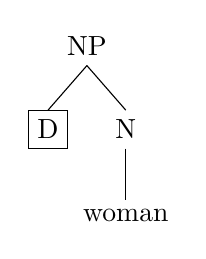
\begin{tikzpicture}
    \Tree 
      [.NP 
        [.\node[draw]{D}; ] 
        [.N [.woman ] ] 
      ] 
  \end{tikzpicture}
  \end{subfigure}
  \caption{TAG productions}
\end{figure}

\begin{figure}[h]
  \centering
  \begin{tikzpicture}
    \begin{scope}[shift={(1.5in,0.80in)}]
    \Tree 
      [.S 
        [.\node(mary-connect){NP}; ] 
        [.VP 
          [.V [.loves ] ] 
          [.\node(woman-connect){NP}; ] 
        ] 
      ] 
    \end{scope}

    \begin{scope}[shift={(0in,0.40in)}]
    \Tree 
      [.\node(mary){NP}; [.N [.Mary ] ] ] 
    \end{scope}

    \begin{scope}[shift={(3.5in,0.0in)}]
    \Tree 
      [.\node(a){D}; [.a ] ] 
    \end{scope}

    \begin{scope}[shift={(4.5in,0.59in)}]
    \Tree 
      [.\node(woman){NP}; 
        [.\node(a-connect){D}; ] 
        [.N [.woman ] ] 
      ] 
    \end{scope}

    \draw[thick,dashed,<-] (mary)..controls +(north:3) and +(south:3)..(mary-connect);
    \draw[thick,dashed,<-] (a)..controls +(north:1.1) and +(south:1.5)..(a-connect);
    \draw[thick,dashed,<-] (woman)..controls +(north:2.5) and +(south:3)..(woman-connect);

  \end{tikzpicture}
  \vspace{-16mm}
  \caption{TAG fragment combination giving parse for ``Mary loves a woman''}
\end{figure}


\begin{figure}[h]
  \centering
  \begin{subfigure}[b]{0.45\textwidth}
  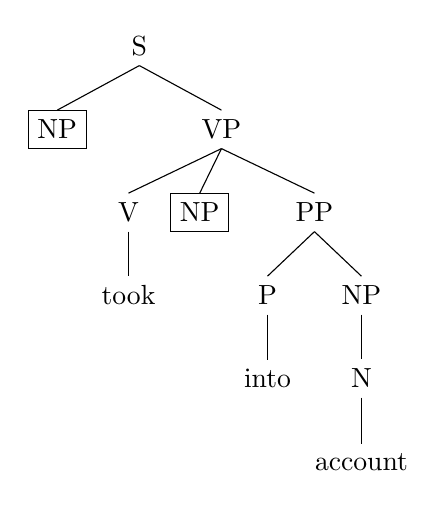
\begin{tikzpicture}
    \Tree 
      [.S 
        [.\node[draw]{NP}; ] 
        [.VP 
          [.V [.took ] ] 
          [.\node[draw]{NP}; ] 
          [.PP
            [.P into ] [.NP [.N account ] ] 
          ] 
        ] 
      ] 
  \end{tikzpicture}
  \end{subfigure}
  \begin{subfigure}[b]{0.30\textwidth}
  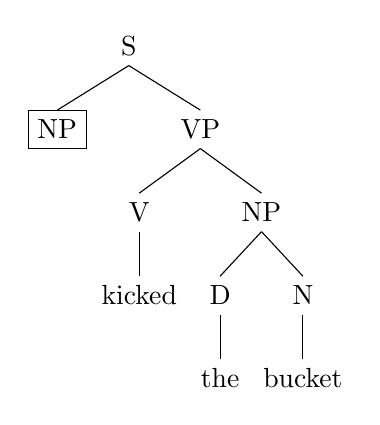
\begin{tikzpicture}
    \Tree 
      [.S 
        [.\node[draw]{NP}; ] 
        [.VP 
          [.V [.kicked ] ] 
          [.NP
            [.D the ] [.N bucket ] 
          ] 
        ] 
      ] 
  \end{tikzpicture}
  \end{subfigure}%
  \caption{TAG productions for common phrases}
\end{figure}




\newpage
\subsection{CCG: Combinatory Categorial Grammar}

\begin{itemize}
  \item Instead of atomic POS tags and Non-Terminals, use \textit{categories} that are constructed from other categories:
	\begin{itemize}
	  \item Categories are defined by a (context-free) grammar \\
	        atomic categories: C \ra~ \{ S, NP, N \} \\
	        complex categories: C \ra~ \{ C/C, C\bs C \}
	  \item Slash and backslash operators indicate that the category is a function:
		\begin{itemize}
		  \item A/B is a category that looks directly to its \textbf{right} for something of category B, and combines with it to produce an A
		  \item A\bs B is a category that looks directly to its \textbf{left} for something of category B, and combines with it to produce an A
		  \item So B is the \textit{input} to the function, and \textit{A} is the output
		\end{itemize}
	\end{itemize}
  \item Mildly context-sensitive
  \item Weakly equivalent to TAG
\end{itemize}

Words are assigned categories in the \textit{Lexicon}:

\begin{itemize}
  \item[] Mary: NP
  \item[] sleeps: S\bs NP
  \item[] loves: (S\bs NP)/NP
  \item[] a: NP/N
  \item[] woman: N
\end{itemize}

The parse tree for a sentence, then, is the result of doing the combinations:

\begin{figure}[h]
  \centering
  \begin{subfigure}[b]{0.08\textwidth}
  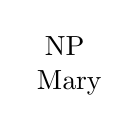
\begin{tikzpicture}[text width=2em,text centered]
    \Tree 
      [.{NP\\Mary} ] 
  \end{tikzpicture}
  \end{subfigure}
  \begin{subfigure}[b]{0.4\textwidth}
  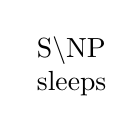
\begin{tikzpicture}[text width=2em,text centered]
    \Tree 
      [.{S\bs NP\\sleeps} ] 
  \end{tikzpicture}
  \end{subfigure}%
  \begin{subfigure}[b]{0.2\textwidth}
  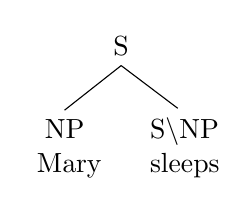
\begin{tikzpicture}[text width=2em,text centered,sibling distance=5mm]
    \Tree 
      [.S
        [.{NP\\Mary} ] 
        [.{S\bs NP\\sleeps} ] 
      ] 
  \end{tikzpicture}
  \end{subfigure}%
  \caption{Series of CCG combinations to parse ``Mary sleeps''}
\end{figure}

\begin{figure}[h]
  \centering
  \hspace{-30mm}
  \begin{subfigure}[b]{0.08\textwidth}
  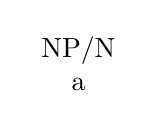
\begin{tikzpicture}[text width=3em,text centered]
    \Tree 
      [.{NP/N\\a} ] 
  \end{tikzpicture}
  \end{subfigure}
  \begin{subfigure}[b]{0.08\textwidth}
  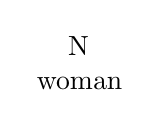
\begin{tikzpicture}[text width=3em,text centered]
    \Tree 
      [.{N\\woman} ] 
  \end{tikzpicture}
  \end{subfigure}
  \begin{subfigure}[b]{0.2\textwidth}
  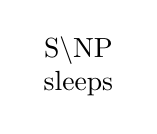
\begin{tikzpicture}[text width=3em,text centered]
    \Tree 
      [.{S\bs NP\\sleeps} ] 
  \end{tikzpicture}
  \end{subfigure}%
  ~
  \begin{subfigure}[b]{0.2\textwidth}
  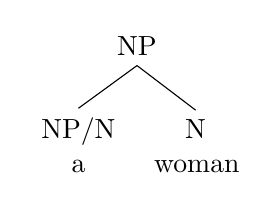
\begin{tikzpicture}[text width=3em,text centered,sibling distance=2mm]
    \Tree 
      [.{NP}
        [.{NP/N\\a} ] 
        [.{N\\woman} ] 
      ] 
  \end{tikzpicture}
  \end{subfigure}%
  \begin{subfigure}[b]{0.2\textwidth}
  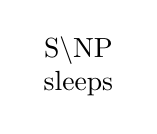
\begin{tikzpicture}[text width=3em,text centered,sibling distance=2mm]
    \Tree 
      [.{S\bs NP\\sleeps} ] 
  \end{tikzpicture}
  \end{subfigure}%
  ~
  \begin{subfigure}[b]{0.1\textwidth}
  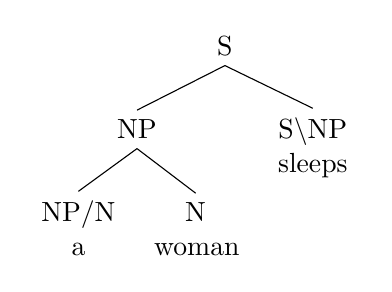
\begin{tikzpicture}[text width=3em,text centered,sibling distance=2mm]
    \Tree 
      [.S
        [.{NP}
          [.{NP/N\\a} ] 
          [.{N\\woman} ] 
        ] 
        [.{S\bs NP\\sleeps} ] 
      ] 
  \end{tikzpicture}
  \end{subfigure}%
  \caption{Series of CCG combinations to parse ``a woman sleeps''}
\end{figure}

\begin{figure}[h]
  \centering
  \begin{subfigure}[b]{0.2\textwidth}
  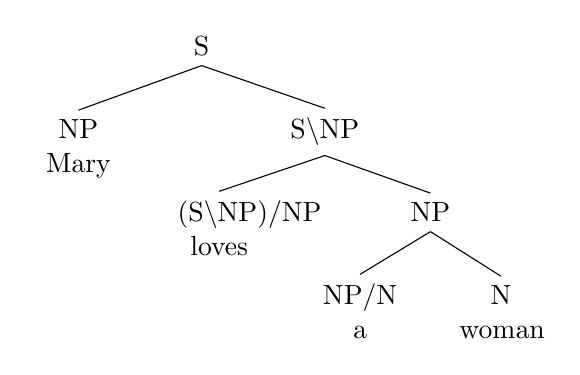
\begin{tikzpicture}[text width=3em,text centered,sibling distance=5mm]
    \Tree 
      [.S
        [.{NP\\Mary} ] 
        [.{S\bs NP} 
          [.{(S\bs NP)/NP\\loves} ]
          [.{NP} 
            [.{NP/N\\a} ]
            [.{N\\woman} ] 
          ] 
        ] 
      ] 
  \end{tikzpicture}
  \end{subfigure}%
  \caption{CCG parse tree for ``Mary loves a woman''}
\end{figure}



\subsection{Dependency Parsing}

\begin{figure}[h]
  \centering
  \begin{subfigure}[b]{0.4\textwidth}
  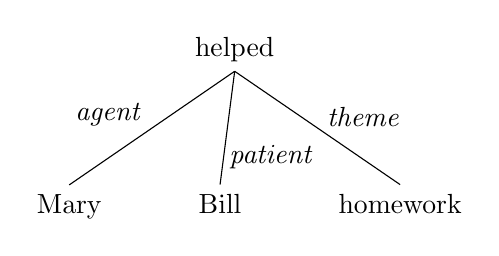
\begin{tikzpicture}

  \tikzset{level distance=20mm, sibling distance=10mm}
    \Tree
      [.helped 
        \edge node[auto=right, yshift=-1mm]{\textit{agent}}; [.{Mary} ]
        \edge node[auto=left,  yshift=-1mm, xshift=-1mm]{\textit{patient}}; [.{Bill} ]
        \edge node[auto=left,  yshift=-1mm]{\textit{theme}}; [.{homework} ]
      ]
  \end{tikzpicture}      
  \caption{``Mary helped Bill with homework.''}
  \end{subfigure}%
  ~~~~~~~ ~~
  \begin{subfigure}[b]{0.4\textwidth}
  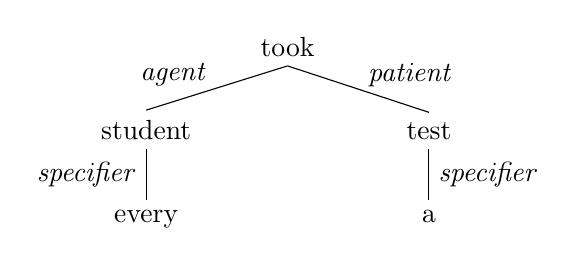
\begin{tikzpicture}
  \tikzset{sibling distance=25mm}
    \Tree
      [.took 
        \edge node[auto=right, yshift=-1mm]{\textit{agent}}; [.{student} 
          \edge node[auto=right]{\textit{specifier}}; [.{every} ] ]
        \edge node[auto=left, yshift=-1mm]{\textit{patient}}; [.{test}
          \edge node[auto=left]{\textit{specifier}}; [.{a} ] ]
      ]
  \end{tikzpicture}      
  \caption{``Every student took a test.''}
  \end{subfigure}
  \caption{Dependency parse trees}
\end{figure}





\end{document}

